\chapter{Структурные свойства задачи оптимизации направленности фазированных антенных решеток} \label{sec:exp}

\section{Постановка вычислительного эксперимента}

Процедура решения задачи оптимизации ФАР при ограничении мощности по каждой точке питания состоит в следующем:
%
\begin{enumerate}
  \item Для каждого излучателя в решетке рассчитать парциальные компоненты полей $f_i^{(l)}, i= \overline{1,N}, l=\overline{1,2}$.
  \item Вычислить матрицы $\textbf{G}$ and $\textbf{H}^{(k)},\ k=\overline{1,n},$ из подраздела~\ref{subsec:statement}.
  \item Оценить радиус допустимой области, используя формулы из подраздела~\ref{subsec:top}.
  \item Решить задачу~(\ref{eq:task3}) с дополнительными ограничениями $x_N = 0, ||\textbf{x}||\le \sqrt{\frac{N}{\lambda_{\min}}}$.
\end{enumerate}

Данный подход может гарантировать нахождение как локального, так и глобального оптимума в зависимости от решателя, используемого на шаге~4. Как один из базовых оптимизационных методов, мы рассматриваем метод градиентной оптимизации (максимизационный вариант)
с алгоритмом одномерного поиска Дэвиса, Свенна и Кэмпи~(ДСК)~\cite{himmelblau:nlp}. Далее целевая функция задачи~(\ref{eq:task3}) будет обозначаться символом $\tilde{F}$.

В нашей работе от задачи условной оптимизации мы переходим к задаче безусловной оптимизации методом штрафных функций, а именно --
методом внешней точки~\cite{eremin:convex,aoki:mo}:
\begin{equation}
       \textbf{x}^{T}\textbf{Gx} - r\cdot \sum_{k=1}^n
       \left( \min\left(0,\textbf{x}^{T}\textbf{H}^{(k)}\textbf{x}\right) +
       \min\left(0,1-\textbf{x}^{T}\textbf{H}^{(k)}\textbf{x}\right)\right)^4 \rightarrow
       \max,
     \label{eq:task4}
\end{equation}
где $r$ -- достаточно большой штрафной параметр. Глобально-оптимальное решение для задачи~(\ref{eq:task4}) может не быть допустимым для изначальной задачи~(\ref{eq:task3}), но увеличение штрафного параметра~$r$ уменьшает нарушение ограничений. Кроме того, имея решение~$\textbf{x}$, которое нарушает в задаче~(\ref{eq:task3}) только неравенства вида $\textbf{x}^{T}\textbf{H}^{(k)}\textbf{x} \leq 1$, мы будем ссылаться на результаты градиентной оптимизации с использованием восстановления допустимости~(\ref{eq:scale}) после срабатывания критерия остановки. Алгоритм градиентной оптимизации повторяется многократно, при этом используется случайно сгенерированный вектор~$\textbf{x}\in \mathbb{R}^{2N}$ в качестве стартовой точки. Распределение случайной величины $\textbf{x}$ описано в подразделе~\ref{subsec:results}. Для каждого найденного решения выполняется проверка на удовлетворение необходимым условиям локальной оптимальности путем решения задачи~(\ref{eq:task5}). Затем решение линеаризованной задачи, удовлетворяющее  необходимым условиям локальной оптимальности, снова подается на вход алгоритма градиентной оптимизации, остальные решения отсеиваются. Последний шаг применяется, поскольку решение задачи~(\ref{eq:task5}) может оказаться за пределами допустимой области задачи~(\ref{eq:task3}). В этом случае данный этап показывает, как далеко решение линеаризованной задачи находится от решения, найденного градиентным алгоритмом. Детальное описание данной процедуры приводится в~\hyperref[sec:applic_a]{приложении~А}.

Для организации вычислительных экспериментов был разработан программный комплекс <<Expi>>~(см.~\hyperref[sec:applic_b]{приложение Б}), зарегистрированный в государственном реестре программ для ЭВМ~\cite{expi}.

С целью отыскания глобального оптимума задачи~(\ref{eq:task3}) посредством решателя BARON~\cite{tawarmalani:global}, основанного на методе ветвей и границ с использованием локальной оптимизации для поиска начального приближения, необходимо предоставить ограничивающий параллелепипед или верхнюю оценку евклидовой нормы допустимых решений. Для этого может быть использовано неравенство~(\ref{eqn:bound}).

\subsection{Тестовые примеры}\label{subsec:examples}

Вычислительный эксперимент был поставлен для задач, построенных на основе четырех типов ФАР: широкополосных вертикальных излучателей, широкополосных вертикальных диполей и симметричных вертикальных диполей. При моделировании полей был использован пакет NEC2, для которого были предоставлены соответствующие геометрические конфигурации антенных систем. В качестве рабочей частоты было выбрано 5МГц. Рассмотрены квадратные ФАР конфигурации 2x2, 3x3 и 5x5. Заранее отметим, что конфигурация 5x5 была рассмотрена только для решеток СВД, поскольку NEC2 не смог обработать 5x5~ШВИ и 5x5~ШВД из-за высокой сложности этих моделей. В случае с ФАР кольцевой структуры были рассмотрены решетки, состоящие из 8 и 16 излучателей.

Решетки ШВИ смоделированы расположенными на высоте 0.2 метра над поверхностью земли (проводимость земли равна~0.01~См/м, относительная диэлектрическая проницаемость~10). Решетки ШВИ и СВД размещены в свободном пространстве. В случае ШВЕ и ШВД, расстояние между соседними излучателями равно 20~метров. Высота каждого излучателя ШВИ равна 15~метров. Расстояние между концами каждого излучателя ШВД равно 30 метров. В случае СВД были рассмотрены два типа излучателя: с длинами излучателя~10~и~30~метров и расстояниями между соседними излучателями 5 и 10 метров соответственно. СВД с длиной излучателя равной 10~метрам в исследовании помечены штрихом (СВД'). Система противовесов ФАР кольцевой структуры поднята над землей на 2м для того, чтобы ослабить влияние потерь в земле. Расстояние между соседними излучателями в этих ФАР равно 8м. В качестве направления максимизации излучения выбраны: азимутальный угол $45^{\circ}$, полярный угол $70^{\circ}$.

\subsection{Результаты вычислительного эксперимента} \label{subsec:results}

В этом разделе мы сравниваем результаты работы градиентного метода и решателя BARON в его режиме по умолчанию. Во всех экспериментах, описанных ниже, было установлено ограничение по времени 1000с. Все эксперименты проводились на ЭВМ с процессором Intel i7 (тактовая частота: 2.8ГГц), ОЗУ: 16Гб. В случае сходимости градиентного метода (завершение по минимально допустимому приращению целевой функции $10^{-4}$) алгоритм перезапускается заново до истечения запаса времени.

Для каждой задачи была применена процедура получения верхней оценки нормы допустимых решений~(c.м. подраздел \ref{subsec:top}). При выполнении этой процедуры для многих задач получались близкие к нулю (или даже нулевые) собственные числа, что делало невозможным их дальнейшее использование для оценки нормы $\sqrt{\frac{N}{\lambda_{\min}}}$. В таблице~\ref{tab:results} такие оценки задачи отмечены прочерком в соответствующем столбце. Так как из физических соображений собственные числа должны быть строго больше 0, проблемы с вычислением верхней оценки нормы допустимых решений свидетельствуют о допущенной погрешности при вычислении матриц, определяющих квадратичные формы задачи~(\ref{eq:task3}). В частности, одной из таких проблем является несимметричный вид вещественных матриц. В таком случае их следует привести к симметричному ввиду путем усреднения симметричных относительно главной диагонали компонент.

Во время каждой инициализации градиентного метода стартовая точка~$\textbf{x}$ выбирается независимо с равномерным распределением в кубе $[-5000, 5000]^{2N}$. Такой выбор оказался достаточным для всех задач, кроме СВД~2x2, чтобы получить решение, по целевой функции соответствующее решению, предоставляемому решателем BARON. Лучшее из найденных таким образом решений принимается за конечный результат. Параметр штрафа~$r$ в методе градиентной оптимизации установлен равным $10^6$ на всех запусках. Такое значение было определено эмпирически. В таблице~\ref{tab:results} приводятся результаты вычислительного эксперимента. Значения целевой функции ``$\tilde{F}$'' в точке, полученной алгоритмом градиентного подъема, приводятся после процедуры масштабирования~(\ref{eq:scale}). Для решателя BARON версии~18.5.8 было выбрано то же самое ограничение сверху на процессорное время, что и для градиентного метода (группа колонок ``BARON''), и 50000с для проверки глобальной оптимальности. Во всех таблицах колонка ``t'' содержит время до получения лучшего найденного решения или до установления глобальной оптимальности. Во всех запусках градиентного метода были получены решения, где активными оказались все ограничения вида $\textbf{x}^{T}\textbf{H}^{(k)}\textbf{x} \leq 1$.

\begin{table}[!h]
\centering
\caption{ Результаты оптимизации, полученные с помощью градиентного подъема и коммерческого решателя}
\begin{tabular}{|c|c|c c|c c|}
    \hline
    \multirow{2}{*}{\textbf{Тип}} & \multirow{2}{*}{$\sqrt{\frac{N}{\lambda_{\min}}}$} & \multicolumn{2}{c}{\textbf{Град.}} & \multicolumn{2}{|c|}{\textbf{BARON}}\\
    & & \textbf{$\tilde{F}$} & \textbf{t, c} & \textbf{$\tilde{F}$} & \textbf{t, c} \\
    \hline
    ШВИ 2х2 & 13.6 & 138.2 & \textbf{0.054} & \textbf{139.2} & 0.12 \\
    ШВИ 3х3 & 22.5 & 575.7 & 0.93 & \textbf{580.6} & \textbf{0.34} \\
    ШВД 2х2 & 21 & 459.7 & \textbf{0.13} & \textbf{463.6} & 0.27 \\
    ШВД 3х3 & 82.2 & 915 & 24.4 & \textbf{925} & \textbf{0.34}  \\
    СВД 2х2 & 44.7& 357 & 1.9 & \textbf{361} & \textbf{0.16} \\
    СВД 3х3 & 641.9& 1138 & 25.6 & \textbf{1261} & \textbf{0.38}\\
    СВД 5х5 & $1.1\cdot10^{5}$ & 5318 & 1000 & \textbf{6716} & 1000 \\
    СВД' 2х2 & $2.3\cdot10^{4}$ & 233 & 2.52 & \textbf{253} & \textbf{0.25} \\
    СВД' 3х3 & $6\cdot10^5$& 664 & 71 & \textbf{1153} & \textbf{1.48} \\
    СВД' 5х5 & - & \textbf{1382.7} & 1000 & 33.5 & \textbf{217.94}  \\
    Кольц. 8 & 87 & 217 & 8.06 & \textbf{218} & \textbf{0.23} \\
    Кольц. 16 & 154 & 727 & 90.9 & \textbf{734} & \textbf{1.37} \\
    \hline
\end{tabular}
\label{tab:results}
\end{table}

Из таблицы~\ref{tab:results} видно, что на всех видах решеток, кроме решеток СВД конфигураций~3x3 и~5x5, а также СВД' конфигураций~2x2 и~3x3, разница в значениях целевой функции не превосходит 1\%. Для решеток СВД конфигураций~3x3 и~5x5, а также СВД' конфигураций~2x2 и~3x3 градиентный алгоритм существенно уступает по качеству найденного решения. Более детальное исследование для СВД' конфигураций 2x2 и 3x3 показало, что BARON предоставляет решение с очень малой областью притяжения. Суть такого исследования заключалась в том, что к решению, полученному с помощью решателя BARON, добавлялось некоторое возмущение, после чего модифицированная точка подавалась на вход градиентного алгоритма. Очень малые возмущения (до 0.5\% относительно нормы решения) исходной точки не мешали градиентному алгоритму найти точку, лежащую в окрестности решения, найденного с помощью решателя BARON. Однако принимая на вход возмущенное порядка 0.5\% относительно нормы решение решателя BARON, градиентный подъем приводил к решению со значением целевой функции $\tilde{F} = 233$  в случае СВД'~2x2. При этом, используемая нами процедура проверки локальной оптимальности не дала опровержения локальной оптимальности решения со значением целевой функции $\tilde{F} = 253$, предоставленного решателем BARON. Аналогичные результаты были получены как для СВД, так и для СВД' конфигурации~3x3.

Особое внимание привлекают решетки СВД и СВД' конфигурации 5x5, поскольку за предоставленный временной промежуток градиентный подъем так и не достиг критерия остановки. BARON в случае СВД'~5x5 за это же время достиг решения, значительно хуже по целевой функции. Вероятно, как BARON, так и градиентный подъем сошлись бы к более качественному решению, если бы не были ограничены по времени.

Кроме решeток ШВИ и ШВД конфигурации~2x2, BARON демонстрирует лучшее время счета. Однако следует отметить, что для обоих алгоритмов время, затраченное на поиск решения, было либо существенно меньше, либо сравнимо со временем, затраченным на построение исходных данных пакетом моделирования NEC, что делает оба подхода равноценными по времени работы с практической точки зрения.

Важным результатом, не приведенным в таблице~\ref{tab:results}, является то, что для ФАР конфигураций ШВИ~2x2, ШВД~2x2 и ШВИ~3x3 была доказана глобальная оптимальность найденного решателем BARON решения.

В качестве иллюстрации физических свойств полученных решений на рис.~\ref{ris:bve_comp} приведен горизонтальный план диаграммы направленности ФАР для решений, найденных с помощью метода градиентной оптимизации. Под диаграммой направленности понимается графическое представление зависимости коэффициента усиления антенны от ее направления в заданной плоскости. Такая диаграмма позволяет наглядно оценить, на какое направление приходится максимум излучения, и провести качественную оценку работы алгоритма. На рис.~\ref{ris:bve_comp} изображена диаграмма направленности для решетки ШВИ размера 2x2 (пунктирная линия) и ШВИ 3x3 (сплошная линия). Для решений, полученных с помощью решателя BARON для этих задач, диаграммы аналогичны. Еще раз отметим, что при эксперименте направление оптимизации было представлено углами в полярных координатах: азимутальный угол был принят равным $45^{\circ}$, полярный угол - $70^{\circ}$. Как видно из горизонтального плана диаграммы направленности при значении полярного угла $70^{\circ}$, максимальному излучению соответствует направление оптимизации $45^{\circ}$. Сравнение диаграмм показывает, что использование решеток с большим числом излучателей позволяет уменьшить излучение в других направлениях.

\begin{figure}[h]
    \centering
    \center{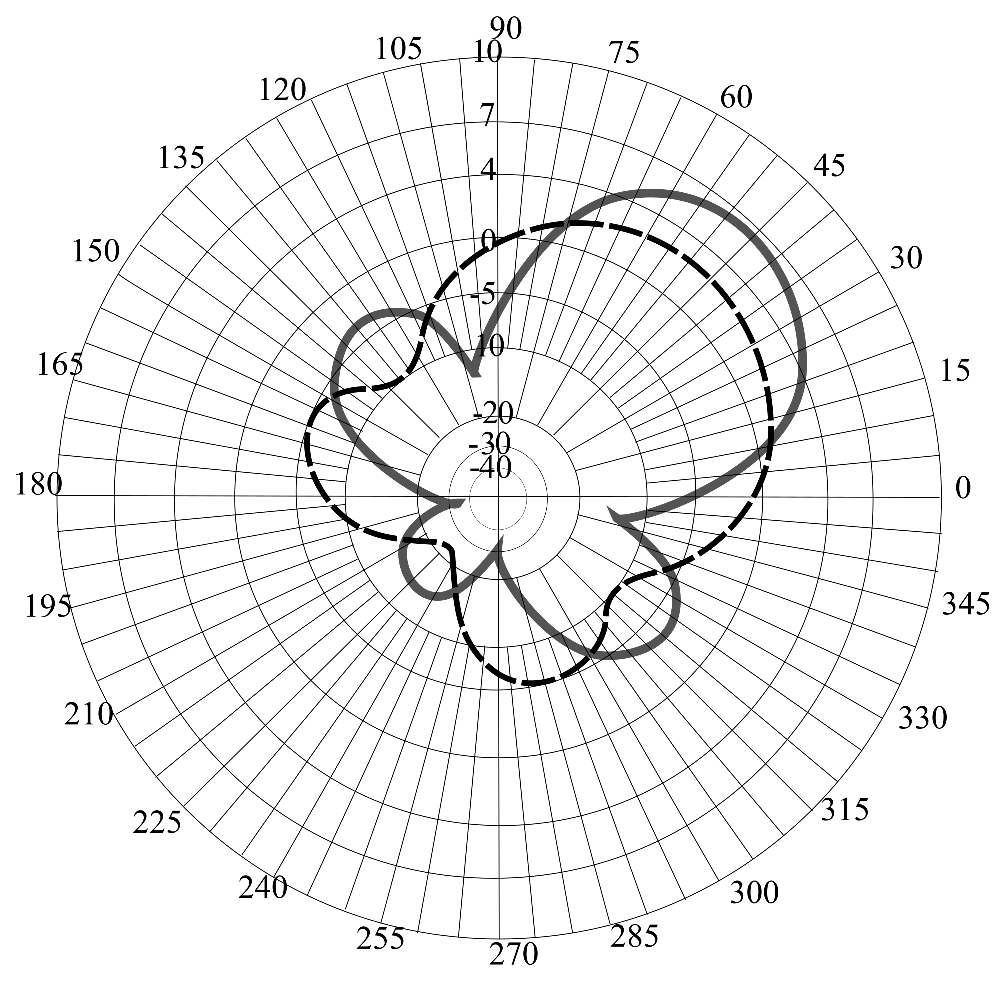
\includegraphics[width=0.5\linewidth]{BWE_comp.eps} }
    \vspace{0.7em}
    \caption{Горизонтальный план диаграммы направленности для решетки ШВИ 2x2 (пунктир) и ШВИ 3x3 (сплошная)}
    \label{ris:bve_comp}
\end{figure}

\section{Количество локальных оптимумов и их расположение}\label{subsec:analyzeloc}
\begin{table}[!h]
\centering
    \caption{Оценки числа локальных оптимумов.}
    \label{tab:structure}
\begin{tabular}{|l | l l | c c c | c c c|}
    \hline
    \textbf{ФАР} & \textbf{$M$} & \textbf{$M_{ne}$} & \textbf{$M_{f}$} & \textbf{$\mathcal{B}_{M_f}$} & \textbf{$\mathcal{L}_{M_f}$} & \textbf{$M_{y\approx0}$} & \textbf{$\mathcal{B}_{M_{y\approx0}}$} & \textbf{$\mathcal{L}_{M_{y\approx0}}$}\\
    \hline
    ШВИ 2x2 & 18368 & 4 & 1 & 1 & 1 & 4 & 4 & 4\\
    ШВД 2x2 & 7678  & 4 & 1 & 1 & 1 & 4 & 4 & 4\\
    СВД 2x2  & 523  & 1 & 1 & 1 & 1 & 1 & 1 & 1\\
    СВД 3x3  & 39  & 9 & 2 & 2 & 2 & 5 & 5 & 5\\
    СВД' 2x2  & 396  & 370 & 3 & 3 & 3 & 338 & 1000 & 1213\\
    СВД' 3x3  & 14  & 14 & 3 & 3 & 3 & 1 & 1 & 1\\
    ШВИ 3x3 & 1070  & 3 & 1 & 1 & 1 & 3 & 3 & 3 \\
    ШВД 3x3 & 41  & 4 & 4 & 4 & 4 & 1 & 1 & 1 \\
    Кольц. 8 & 124  & 9 & 2 & 2 & 2 & 9 & 9 & 9\\
    Кольц. 16 & 11  & 6 & 1 & 1 & 1& 6 & 6 & 6\\
    \hline
\end{tabular}
\end{table}

\begin{figure}
\centering
    \begin{minipage}[h]{0.8\linewidth}
            \center{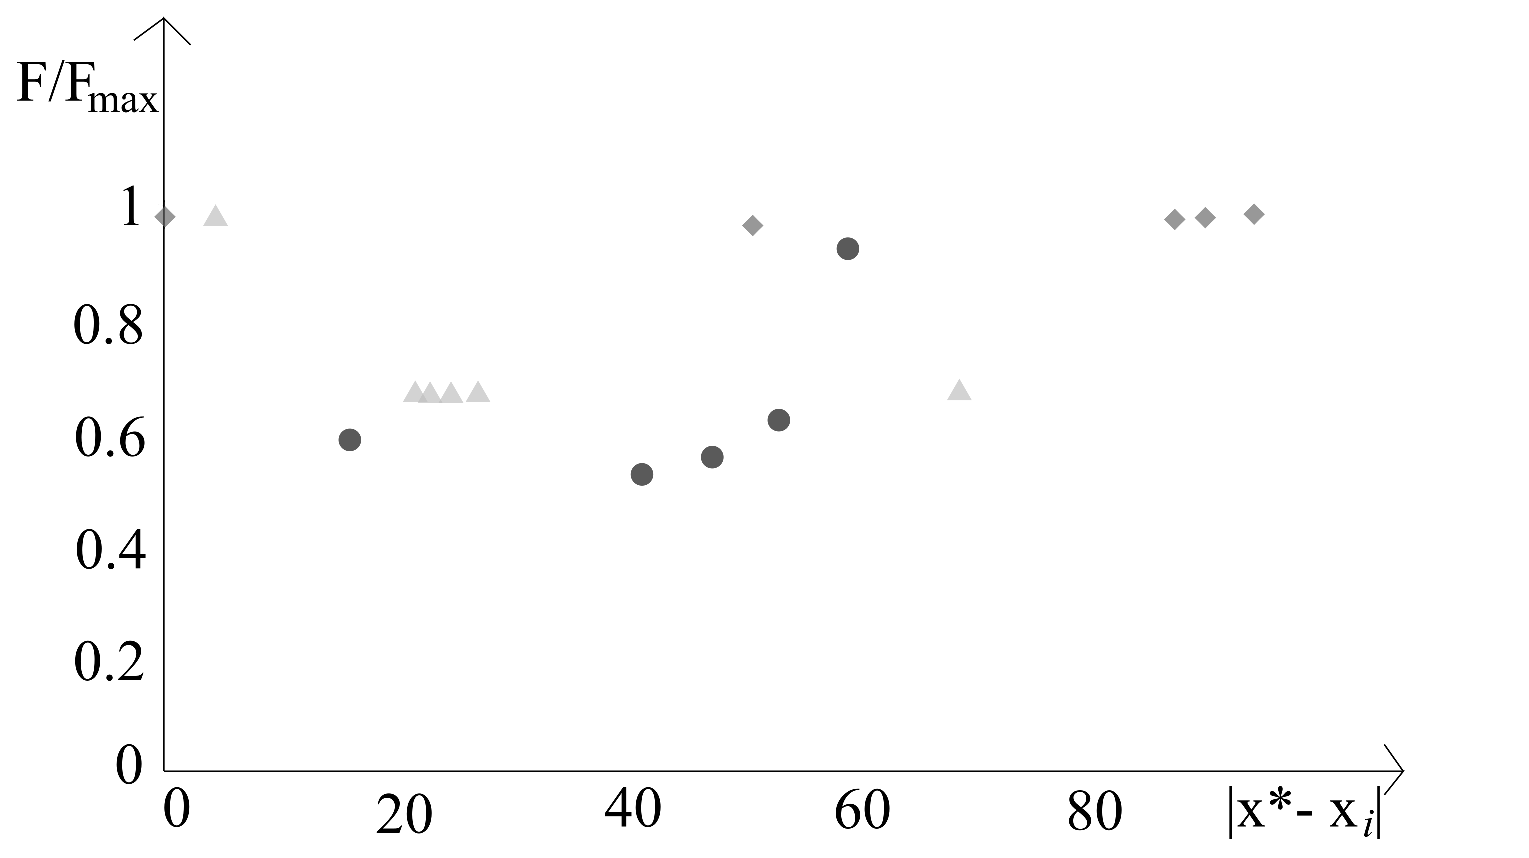
\includegraphics[width=0.9\linewidth]{fit_dist.eps}  \\ а) }
    \end{minipage}
    \begin{minipage}[h]{0.8\linewidth}
            \center{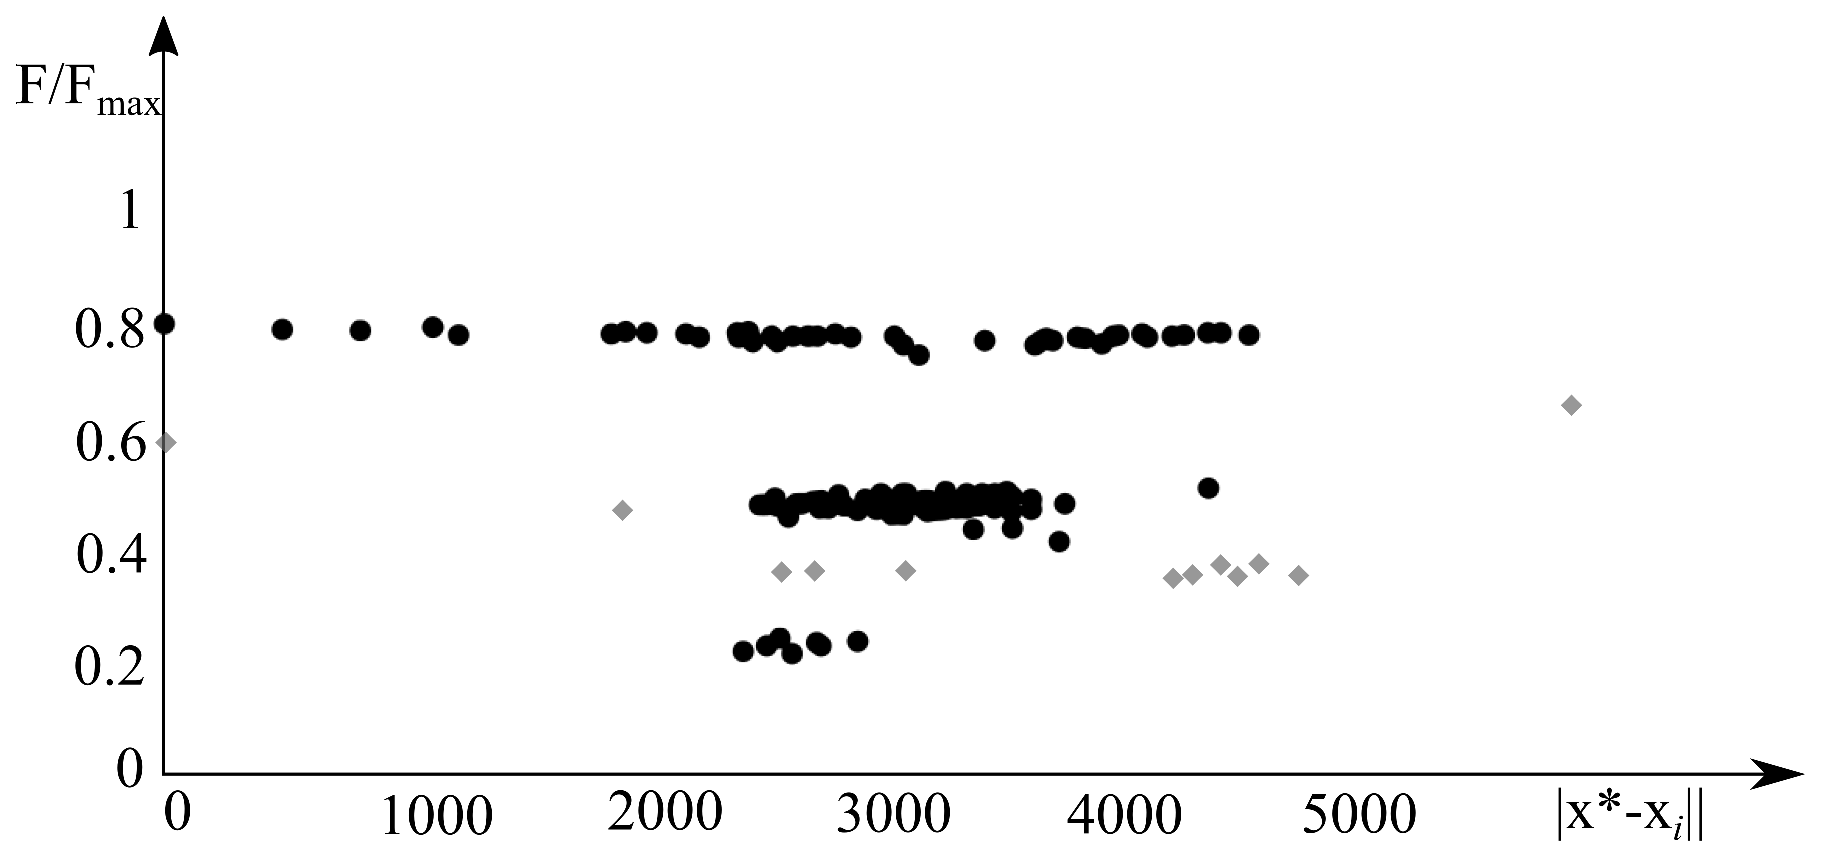
\includegraphics[width=0.9\linewidth]{fit_dist_2x2.eps}  \\ б) }
    \end{minipage}
    \vspace{0.7em}
    \caption{Структура множества найденных решений. В случае а) точками обозначены результаты для кольцевых решеток, состоящих из 8 излучателей, ромбами -- для кольцевых решеток, состоящих из 16 излучателей, треугольниками - для СВД~3x3. В случае б) точками обозначены результаты для СВД'~2x2, ромбами -- для СВД'~3x3}
    \label{ris:fit_dist}
\end{figure}

Для оценки общего числа локальных оптимумов использовался метод переписи Шнабеля. Данный метод имеет применение в экологии и заключается в
выводе статистических оценок численности популяции на основе числа особей, помеченных в результате эксперимента, из популяции с неизменным
составом, где каждая особь имеет константную вероятность отлова. В~\cite{eremeev:confidence} предлагается адаптация такого метода для оценки числа локальных оптимумов.

В таблице~\ref{tab:structure} приводится статистика по числу различных точек остановки (в пределах заданной точности) процедуры мультистарта в течение 1000с процессорного времени. Для каждого решения была применена процедура линеаризации задачи и проверки необходимых условий локальной оптимальности, описанная в разделе~(\ref{sec:loc}). Приемлемыми считались отличия целевой функции линеаризованной задачи от значения целевой функции, найденного градиентным методом, менее чем на 1\%. Здесь {$M$} -- число выполненных запусков за отведенное время, $M_{ne}$ -- число групп решений, отличающихся не более чем на 10\% по каждой из координат, {$M_{f}$} -- число групп значений целевой функции у таких неэквивалентных решений (с точностью до 10\%, приведенных в таблице~\ref{tab:results}). {$M_{y\approx0}$} -- число групп решений, для которых были выполнены необходимые условия локальной оптимальности~(см.~\S~\ref{sec:loc} ниже). $\mathcal{B}$ и $\mathcal{L}$ -- оценка нижней границы и оценка максимального правдоподобия числа локальных оптимумов, рассчитанные по методу переписи Шнабеля. Доверительная вероятность для данного метода была выбрана равной 95\%. Оценки для числа решений с различными значениями целевой функции обозначены $\mathcal{B}_{M_f}$ и $\mathcal{L}_{M_f}$. Оценки для числа решений, для которых были выполнены необходимые условия локальной оптимальности, обозначены $\mathcal{B}_{M_{y\approx0}}$ и $\mathcal{L}_{M_{y\approx0}}$.
В случае СВД и СВД' конфигурации 5x5 в течение 1000~с градиентный метод не достиг решения, удовлетворяющего условию остановки, поэтому
данный результат не включен в таблицу~\ref{tab:structure}.

Как видно из таблицы, во всех экспериментах в некоторых запусках были найдены неразличимые с практической точки зрения решения. Для квадратных решеток ШВИ и ШВД было найдено по одному такому решению. Решетки кольцевой структуры и СВД'~2x2 имеют значительное разнообразие как по найденным векторам решений, так и по значениям целевой функции. Относительно решений, для которых были выполнены необходимые условия локальной оптимальности, можно сказать, что, с большой вероятностью, для задачи СВД'~2x2 были найдены далеко не все возможные решения. О решетке СВД'~3x3 известно, что градиентный подъем был остановлен в точке, не лежащей в окрестности решения, предоставляемого решателем BARON.

На рис.~\ref{ris:fit_dist} приведены диаграммы локальных оптимумов, где по оси ординат отложены значения целевой функции, а по оси
абсцисс - расстояние до лучшего известного решения. Диаграмма показывает, что значения, соответствующие одному и тому же значению целевой функции, могут находиться достаточно далеко друг от друга, что позволяет сделать предположение о наличии неучтенных симметрий задачи (о множестве линейных симметрий задачи см. в~\cite{yurkov:symmetry}).

\section{Проверка необходимых условий локальной оптимальности} \label{sec:loc}

Как уже было отмечено, нахождение даже локального оптимума в случае решения задачи невыпуклого квадратичного программирования, вообще говоря, является NP-трудным. В связи с этим применительно к градиентному подъему можно ожидать ситуаций, в которых при поиске локального оптимума потребуется чрезмерно большое число итераций или произойдет преждевременная остановка вдалеке от локального оптимума. Из этого следует, что имеет смысл предусмотреть процедуру, позволяющую определить случаи, когда полученное решение не является локальным оптимумом. Для этого была применена процедура проверки необходимых условий локальной оптимальности~\cite{murty:np}. Суть данной проверки в том, что мы линеаризуем задачу вблизи точки остановки градиентного алгоритма. Для этого в окрестности решения $\textbf{x}_0$ вводим малое приращение $\textbf{у}$. При этом каждая квадратичная форма, представленная симметричной матрицей $\textbf{M}$, преобразуется следующим образом:
$$\textbf{x}^T\textbf{M}\textbf{x} = \textbf{x}_0^T\textbf{M}\textbf{x}_0 +
\textbf{x}_0^T\textbf{M}\textbf{y} + \textbf{y}^T\textbf{M}\textbf{x}_0 +
\textbf{y}^T\textbf{M}\textbf{y}.$$ Учитывая симметричность каждой квадратичной формы и пренебрегая квадратичными по $\textbf{y}$ слагаемыми, получаем для задачи~(\ref{eq:task3}):


\begin{equation}
    \begin{cases}
       \textbf{x}_0^T\textbf{G}\textbf{x}_0 + 2\textbf{x}_0^T\textbf{G}\textbf{y} \rightarrow \max,\\
       0 \leq \textbf{x}_0^T\textbf{H}^{(1)}\textbf{x}_0 + 2\textbf{x}_0^T\textbf{H}^{(1)}\textbf{y} \leq 1,\\
       ...\\
       0 \leq \textbf{x}_0^T\textbf{H}^{(n)}\textbf{x}_0 + 2\textbf{x}_0^T\textbf{H}^{(n)}\textbf{y} \leq 1,\\
      \textbf{y} \in \mathbb{R}^{2N}.\\
     \end{cases}
     \label{eq:task5}
\end{equation}

В случае локальной оптимальности решения $\textbf{x}_0$ модуль $|\textbf{y}^T\textbf{G}\textbf{y}|$ должен быть равен нулю.

Следует отметить, что решение задачи~(\ref{eq:task5}) не подтверждает локальную оптимальность, а лишь предоставляет вспомогательную процедуру, благодаря которой из всего множества решений, найденных в результате многократного запуска из случайно сгенерированной точки
градиентного подъема, можно исключить решения, заведомо не являющиеся локальными оптимумами. Такие решения могут быть получены в результате преждевременного завершения работы градиентного метода по точности, если значения целевой функции слабо меняются за итерацию алгоритма или текущее решение оказалось в стационарной точке, не являющейся локальным оптимумом (последнее случается крайне редко).

\section{Экспериментальная проверка устойчивости решений}
\begin{figure}[h]
    \centering
    \center{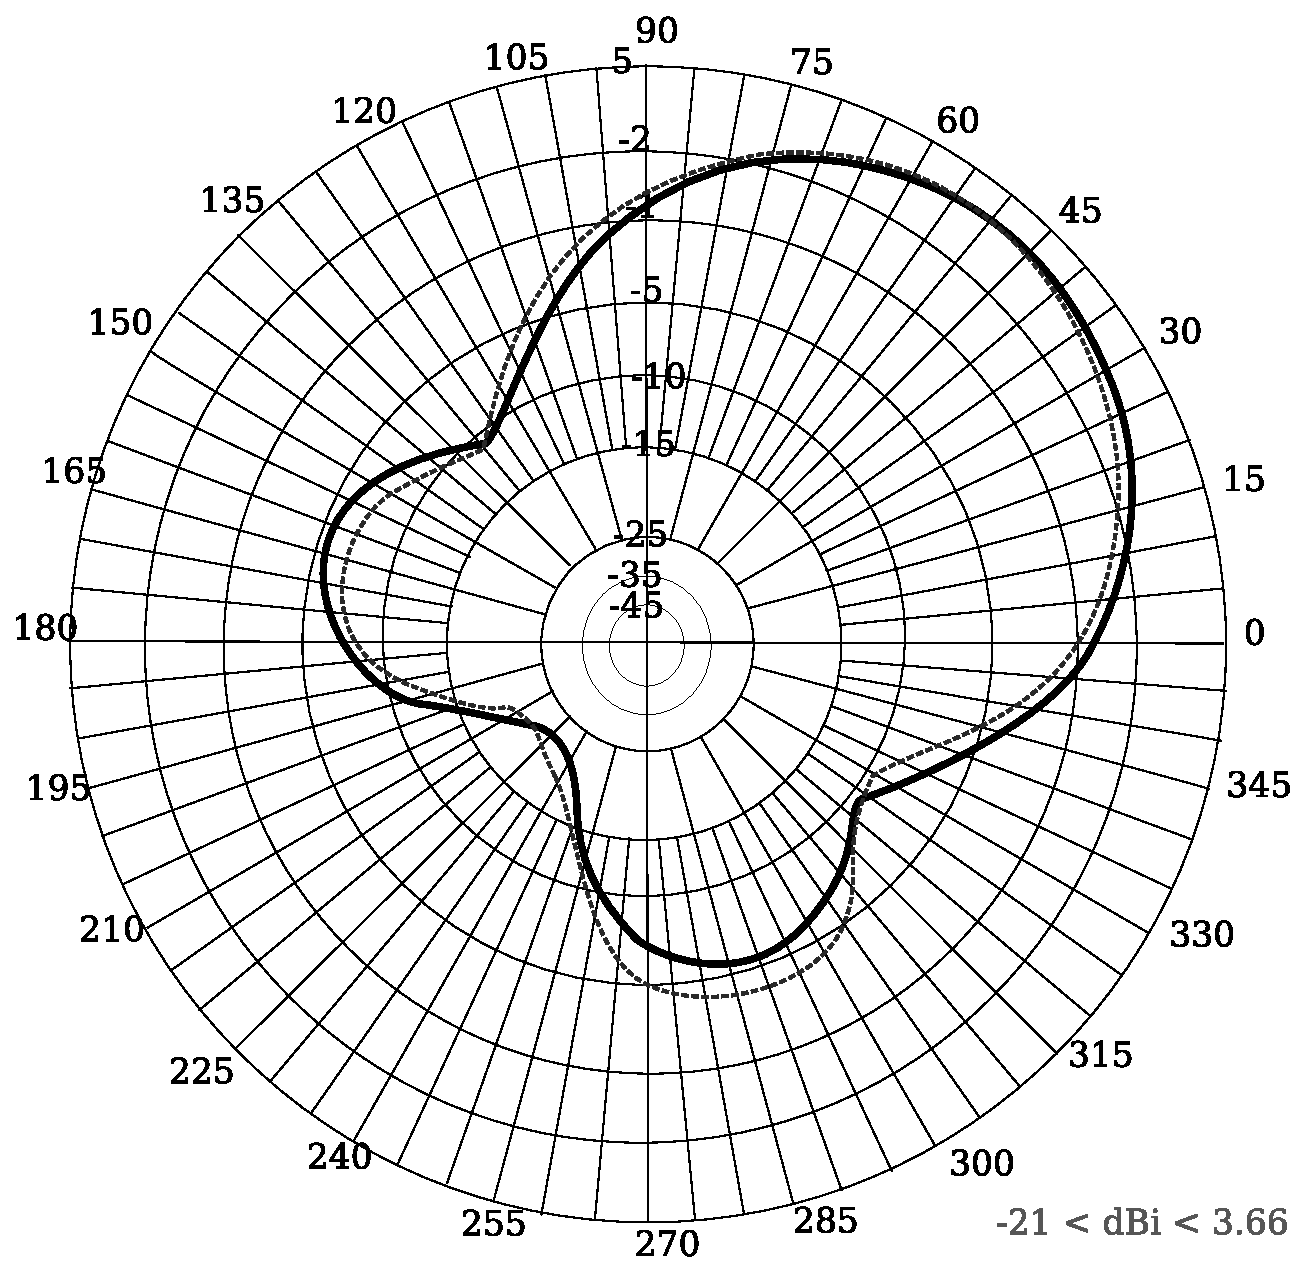
\includegraphics[width=0.5\linewidth]{stability.eps} }
    \vspace{0.7em}
    \caption{Диаграммы направленности для ШВИ~2x2 при оптимизации в направлении 70:45 (сплошная линия) и 70:50 (пунктир)}
    \label{ris:bve_comp}
\end{figure}
При анализе структуры локальных оптимумов может возникнуть вопрос об устойчивости решения по аргументу. В данной работе было проведено исследование изменения значения целевой функции при изменении оптимизируемого направления на малый угол. В рассмотрение принималось также изменение значения целевой функции при подстановке в исходную задачу решения, найденного для нового направления (для удобства вывода результата такая подстановка обозначена P1), и наоборот -- при подстановке в задачу для измененного направления решения, полученного для исходного направления (обозначается P2). Исследование проводилось на квадратных решетках, состоящих из 4-х и 9-и излучателей. Азимутальный и полярный угол менялись на $5^{\circ}$. Результаты приведены в таблице~\ref{tab:stability}
\begin{table}[!h]
\centering
\begin{tabular}{|c|c|c|c|c|c|c|c|}
    \hline
    \textbf{ФАР} & \textbf{Подстановка} & \textbf{70:45} & \textbf{75:45} & \textbf{65:45} & \textbf{70:50} & \textbf{75:40} & \textbf{65:50}\\
    \hline
    \multirow{3}{*}{ШВИ 2x2} & - & \multirow{3}{*}{138} & 125 & 138 & 137 & 137 & 125\\
    & P1 &  & 138 & 138 & 137 & 137 & 137\\
    & P2 &  & 125 & 138 & 136 & 136 & 123\\
    \hline
    \multirow{3}{*}{ШВИ 3x3} & - & \multirow{3}{*}{575} & 532 & 565 & 574 & 533 & 564\\
    & P1 &  & 574 & 572 & 560 & 558 & 557\\
    & P2 &  & 530 & 562 & 559 & 517 & 546\\
    \hline
    \multirow{3}{*}{ШВД 2x2} & - & \multirow{3}{*}{459} & 518 & 454 & 454 & 512 & 389\\
    & P1 &  & 458 & 459 & 457 & 456 & 389\\
    & P2 &  & 518 & 392 & 452 & 510 & 386\\
    \hline
    \multirow{3}{*}{ШВД 3x3} & - & \multirow{3}{*}{1501} & 1817 & 872 & 1015 & 1196 & 1198\\
    & P1 &  & 1506 & 1047 & 1000 & 1004 & 1448\\
    & P2 &  & 1774 & 1203 & 1450 & 1713 & 1162\\
    \hline
    \multirow{3}{*}{СВД 2x2} & - & \multirow{3}{*}{369} & 417 & 315 & 365 & 412 & 312\\
    & P1 &  & 368 & 369 & 367 & 366 & 367\\
    & P2 &  & 417 & 315 & 363 & 410 & 310\\
    \hline
    \multirow{3}{*}{СВД 3x3} & - & \multirow{3}{*}{1484} & 1789 & 1176 & 1459 & 1162 & 1753\\
    & P1 &  & 1475 & 1472 & 1446 & 1428 & 1444\\
    & P2 &  & 1782 & 1164 & 1427 & 1120 & 1713\\
    \hline
\end{tabular}
    \caption{Значения целевой функции при изменении оптимизируемого направления на малый угол.}
    \label{tab:stability}
\end{table}

Результаты исследования показывают, что изменение направления оптимизации на малый угол соответствует повороту исходной диаграммы направленности на этот угол.

\section{Исследование симметрий задачи}

Для полноты изложения в разделах \ref{sec:sym_common} и \ref{sec:sym_cont} приводятся элементы теории из~\cite{yurkov:symmetry}.
\subsection{Общие положения}
\label{sec:sym_common}
Решение и исследование задач математического программирования могут быть упрощены при наличии симметрий этих задач, соответствующих некоторым линейным преобразованиям. В частности, знание таких симметрий может быть использовано для уменьшения размерности задачи, ограничения пространства поиска или получения нового локального оптимума из имеющегося. Эти методы применимы в
случае непрерывной области решений~\cite{CHL13,GATERMANN200495,KWM19}, а также в целочисленном программировании~\cite{BHJ13,C99,Kolokolov2012,Margot2010,Simanchev96} и частично целочисленном программировании \ \cite{L12,PR19}.
Хотя в большинстве случаев применение симметрий направлено на ускорение работы алгоритмов точной оптимизации, в некоторых случаях знание симметрий может оказаться полезным и при разработке и анализе эвристик, в частности, эволюционных алгоритмов~\cite{Doerr21,Adam2004}.

В настоящей работе исследуется случай непрерывной области решений. В то время как предыдущие исследования симметрии в математическом программировании, как правило, имели дело с перестановками координат пространства решений~\cite{Kolokolov2012,KWM19,L12}, в данной работе рассматривается большая группа обратимых линейных преобразований. Мы изучаем частный случай задачи квадратичного программирования с квадратичными ограничениями в~${\mathbb R}^N$: целевая функция и ограничения задаются квадратичными формами $\textbf{G}, $ и $\textbf{H}_1,\dots,\textbf{H}_n,$ в виде~(\ref{eq:task3}). Следует еще раз отметить, что все матрицы $\textbf{G}, $ и $\textbf{H}_1,\dots,\textbf{H}_n,$ симметричны и $\textbf{H}_\Sigma = \sum_{i=1}^{n}\textbf{H}_i$ положительно определена.
Без потери общности будем считать, что все ограничения заданы неравенствами~$\le$.
Известная задача о максимальном разрезе (которая является NP-трудной) также может быть сведена к задаче квадратичного программирования с такими свойствами~\cite{Shor1998}.

Под симметрией задачи~(\ref{eq:task3}) подразумевается набор линейных преобразований
%of the column space
\begin{equation}
\label{eq:Lin}
\textbf{x} \to \textbf{y}=\textbf{Px} \, ,
\end{equation}
%

определенный невырожденной матрицей $\textbf{P}$, такой что задача~(\ref{eq:task3}), выраженная в терминах преобразованного пространства
(т.е, через вектор-столбец $\textbf{y} $), совпадает с исходной задачей. Таким образом, в терминах вектора $\textbf{y}$ задача~(\ref{eq:task3}) формулируется в той же форме:
%
\begin{equation}
\label{eq:Tinit}
\left\{
\begin{array}{l}
\displaystyle
\textbf{y}^T \textbf{G y} \to {\max} \, , \\
\displaystyle
\textbf{y}^T\textbf{H}_1\textbf{y} \le  1 \, , \\
\displaystyle
\dots \\
\textbf{y}^T\textbf{H}_n\textbf{y} \le 1 \, ,
\end{array}
\right.
\end{equation}
%
\textit{с той же самой} матрицей $\textbf{G} $ и тем же набором матриц $\{\textbf{H}_i: i=1,\dots,n\}$. Подчеркнем, что поскольку перестановка ограничений не меняет задачи, матрицы $\textbf{H}_i$ также могут быть пронумерованы произвольно.

Преобразования, заданные матрицами $\textbf{P}$, составляют группу обратимых линейных симметрий, которую мы обозначаем через~$\mathcal G$. Нахождение хотя бы подгруппы в~$\mathcal G$, также может иметь смысл для практических целей, если полученные симметрии позволяют упростить оптимизационную задачу.

В некоторых случаях также может потребоваться найти группу симметрии только набора ограничений. Обозначим эту группу через~$\mathcal G'$.
Очевидно, это мало чем отличается от поиска группы симметрии~$\mathcal G$ задачи; нужно просто исключить из рассмотрения матрицу $\textbf{G}$ (формально можно считать, что $\textbf{G}$ в этом случае нулевая матрица). Обратите внимание, что $\mathcal G$ является подгруппой в $\mathcal G'$.
{
Кроме того, набор симметрий ограничений тесно связан, но не обязательно идентичен набору тех обратимых линейных преобразований, которые биективно отображают область допустимости задачи ${\mathcal D}:=\{\textbf{x}\in {\mathbb R}^N \ : \ \textbf{x}^T B_i \textbf{x} \le 1, \ i=1,\dots,M\}$ на себя. Группа симметрии множества ограничений~$\mathcal{G}'$ может быть подгруппой в группе симметрии обратимых линейных преобразований области~${\mathcal D}$. Это происходит, например, если имеется несколько ``неактивных'' ограничений, каждое из которых определяет такое множество точек, внутри которого содержится ${\mathcal D}$. Тогда требование, чтобы набор матриц этих ``неактивных'' ограничений оставался в~(\ref{eq:Tinit}), является избыточным относительно группы преобразований области~${\mathcal D}$. В качестве простого примера рассмотрим случай $n=N+1,$ $\textbf{G}={diag}(1,\dots,1), \ \textbf{H}_1={diag}(1,0,0,\dots ,0), \dots, \textbf{H}_N={diag}(0,0,\dots,0,1), \textbf{H}_{N+1}={diag}(1,\dots,1).$ Ясно, что здесь $\textbf{H}_1,\dots,\textbf{H}_N$ определяют ``неактивные'' ограничения, группа обратимых линейных преобразований области~${\mathcal{D}}$ состоит из всех ортогональных преобразований в~${\mathbb R}^N $, а группа $\mathcal G$ — конечная группа линейных симметрий $N$-мерного гиперкуба.
}

Авторы~\cite{GATERMANN200495} объединяют последнее определение симметрии области допустимости с инвариантностью целевой функции для изучения геометрических, алгебраических и вычислительных свойств, подразумеваемых такими (дискретными) симметриями в полуопределенных программах. В этом случае с помощью симметрий получается эквивалентная задача выпуклой оптимизации с меньшим числом переменных и тем же оптимальным решением.

В~\cite{L12} группа формулировок задачи математической оптимизации была определена как множество перестановок индексов переменных, для которых целевая функция и ограничения остаются неизменными. Ясно, что эта группа является подгруппой в $\mathcal{G}$. На основе подхода из~\cite{L12}, в~\cite{KWM19} был разработан алгоритм обнаружения симметрии для задач квадратичного программирования. Этот алгоритм можно использовать для нахождения группы формулировок в нашем случае, однако мы стремимся найти всю группу~$\mathcal{G}$, если это возможно.

Обозначим множество матриц $\textbf{H}_1,\dots,\textbf{H}_n$ через ${\mathcal{H}}$.

\begin{definition} \label{def:invariance}
${\mathcal H}$ называется {\em конгруэнтным инвариантом} (или просто инвариантом, для краткости) относительно преобразования
%
\begin{equation}
\label{transform}
\textbf{H} \to \textbf{P}^T \textbf{H P} \,
\end{equation}
%
с невырожденной матрицей $P$, если $\{P^T \textbf{H} P \ : \ \textbf{H} \in {\mathcal H}\}= \{\mathcal H\}$.
\end{definition}

Множество всех матриц $P$, для которых множество ${\mathcal{Р}}$ является инвариантом, образует группу. Здесь эта группа называется {\em группа симметрий множества матриц}~${\mathcal{Р}}$ и обозначается~${\mathcal{G}}_{\mathcal{H}}$. Ясно, что относительно преобразования $\textbf{H} \to \textbf{P}^T \textbf{H P}$ некоторые матрицы из $\mathcal{H}$ могут сводится к другим, однако не все возможные комбинации могут быть получены этим способом.

Заметим, что одним из инвариантов преобразования~(\ref{transform}) является {\em инерция} матрицы~$\textbf{H}$,
определяется как упорядоченная тройка: (i)~количество положительных собственных значений~$\textbf{H}$, (ii)~количество отрицательных собственных значений~$\textbf{H}$ и (iii)~количество нулевых собственных значений~$\textbf{H}$ (см., например,~\cite{horn:matrix}, \S~4.5). Таким образом, можно переставлять только матрицы с одинаковой инерцией, а все множество ${\mathcal{H}}$ разбивается на классы эквивалентности матриц с одинаковой инерцией. Это отражено в следующем определении.
\begin{definition}
{\em I-класс} является максимальным по включению подмножеством ${\mathcal{H}}$, состоящим из матриц с равной инерцией.
\end{definition}

Предполагается, что все I-классы ${\mathcal{H}}$ пронумерованы целым числом~$k$ и обозначены~${\mathcal{H}}^I_k$. Обозначим
%
\begin{equation}
{\mathcal{H}} = \bigcup_k {\mathcal{H}}^I_k \, .
\end{equation}
%

Кроме того, сумма \textit{всех} матриц, принадлежащих некоторому I-классу, является инвариантом любого преобразования~(\ref{transform}) из ${\mathcal{G}}_{\mathcal{H}} $

Заметим, что это не все инвариантные суммы, поскольку любая сумма нескольких классов инерции также является инвариантом. Таким образом, по множеству $ {\mathcal{H}} $ можно явно построить набор матриц, инвариантных относительно всех преобразований~(\ref {transform}), перебирая все комбинации I-классов и суммируя их элементы.

\begin{definition}
Любая матрица, являющаяся суммой всех матриц, принадлежащих одному или нескольким I-классам, называется {\em матрицей инвариантности I-типа.}
\end{definition}

%Могут существовать и другие матрицы инвариантности, однако способы их нахождения, и проверка их существования в настоящще время не выяснены.

В~\cite{yurkov:symmetry} показано, что можно упростить анализ группы $\mathcal{G}_{\mathcal{B}}$, если хотя бы одна из матриц инвариантности I-типа положительно определена, так как в этом случае мы сможем использовать известные факты о группе ортогональных преобразований~$O(N)$ (см., например,~\cite{Zhelobenko}).

Можно сказать, что

\textbf{Условие I} {\em выполняется, если по меньшей мере одна инвариантная матрица $H^I$ I-типа положительно определена.}

Следует обратить внимание, что симметричная матрица~$\textbf{H}$ может быть представлена как конгруэнтное преобразование диагональной матрицы:
%
\begin{equation}
\label{eq:BSSTDS}
\textbf{H}=\textbf{S}^T\textbf{DS} \, ,
\end{equation}
%
где $\textbf{D}$ -- диагональная матрица, которая может иметь только ``0'', ``1'', или ``-1'' на ее главной диагонали. Матрица $\textbf{S}$ Может быть получена конструктивно, например, конечным методом Лагранжа~(\cite{Lancaster},~Г.~5).

В тех случаях, когда $\textbf{H}$ положительно определена, матрица~$\textbf{D}$ будет являться единичной матрицей и может быть опущена в~(\ref{eq:BSSTDS}).

\begin{proposition} \label{prop:orthogonal} \cite{yurkov:symmetry}~Если условие~I выполняется, тогда группа $ {\mathcal{G}}_{\mathcal{H}} $ является изоморфизмом некоторой подгруппы группы ортогональных преобразований, и этот изоморфизм определяется отображением
\begin{equation}
\label{eq:Qdef_map}
\textbf{P} \to \textbf{SPS}^{-1},
\end{equation}
где матрица $S$ такова, что $\textbf{H}^I=\textbf{S}^T \textbf{S}$.
\end{proposition}

{
Инвариантность задачи~(\ref{eq:task3}) относительно преобразования~$\textbf{P}$ подразумевает, что
%
\begin{equation}
\label{eq:geninvar}
\textbf{P}^T\textbf{GP}=\textbf{G} \,  , \qquad \textbf{P}^T\textbf{H}_i \textbf{P} = \sum_{j=1}^n \textbf{L}_{ij}\textbf{P}_j , \  i=1,\dots,n,
\end{equation}
%
где $ \textbf{L}_{ij} $ -- элементы матрицы перестановок, т.е. матрица ${\textbf{L}=(\textbf{L}_{ij})}$ имеет одну единицу в каждом столбце и в каждой строке, остальные элементы~$\textbf{L}$ равны нулю.

Утверждение~\ref{prop:orthogonal} может быть применено для анализа симметрий задачи~(\ref{eq:task3}), если известны некоторые матрицы инвариантности I-типа $\textbf{H}^I$ для множества матриц ${\mathcal{H}}=\{\textbf{H}_1,\dots,\textbf{H}_n\},$ подразумевая, что
%
\begin{equation}
\label{eq:invBS}
\textbf{P}^T \textbf{H}^I \textbf{P} = \textbf{H}^I,
\end{equation}
и { $\textbf{H}^I$ } положительно определена.

В задаче оптимизации направленности ФАР матрица~$\textbf{H}_{\Sigma}:=\sum_i \textbf{H}_i$ положительно определена. Если выполняется~(\ref{eq:geninvar}), тогда $\textbf{H}^I=\textbf{H}_{\Sigma}$ является матрицей инвариантности I-типа для множества матриц ${\mathcal{H}}=\{\textbf{H}_1,\dots,\textbf{H}_n\}.$

Естественно, в общем случае инвариантность матрицы $\textbf{H}^I$ не обязательно подразумевает выполнение~(\ref{eq:geninvar}), но по крайней мере можно говорить, что группа~$\mathcal G'$ является подгруппой ${\mathcal G}_{\mathcal{B}}$, которая в свою очередь является подгруппой в $O(N)$ по утверждению~\ref{prop:orthogonal}. Следовательно, $\mathcal{G}$ также является подгруппой~$O(N)$.

За $\textbf{Q}$ обозначим ортогональное преобразование вида~(\ref{eq:Qdef}).
\begin{equation}
\label{eq:Qdef}
\textbf{Q}:=\textbf{SPS}^{-1}
\end{equation}

В дальнейшем всегда будем предполагать, что существует положительно определенная инвариантная матрица $\textbf{H}^I$ I-типа для множества матриц ${\mathcal{H}}=\{\textbf{H}_1,\dots,\textbf{H}_n\},$ т.е. условие~I выполнено, и $\textbf{Q}$ всегда будет обозначать образ~$\textbf{P}$ при изоморфизме~(\ref{eq:Qdef_map}).

%This means that the matrix $Q = STS^{- 1} $, generally speaking, belongs to the pseudo-orthogonal group~\cite{Zhelobenko}.

Поскольку $\textbf{P}=S^{-1}\textbf{QS}$ по определению~$\textbf{Q}$, применение~(\ref{eq:geninvar}) дает

%
\begin{equation}
\begin{array}{l}
\displaystyle
(\textbf{S}^{-1}\textbf{QS})^T\textbf{G}(S^{-1}\textbf{QS})=\textbf{G} \,  , \\ \\
\displaystyle
(\textbf{S}^{-1}\textbf{QS})^T\textbf{H}_i (\textbf{S}^{-1}\textbf{QS})= \sum_{j=1}^n \textbf{L}_{ij}\textbf{H}_j \, , \ i=1,\dots,n,
\end{array}
\end{equation}
%

и после простого преобразования получается
%
\begin{equation}
\label{eq:invarwithQ}
\textbf{Q}^T \tilde{\textbf{G}} \textbf{Q}=\tilde{\textbf{G}} \,  , \ \ \ \
\textbf{Q}^T \tilde{\textbf{H}_i} \textbf{Q}= \sum_{i=1}^N \textbf{L}_{ij}\tilde{\textbf{H}_j} \, , \ i=1,\dots,n,
\end{equation}
%
где
%
\begin{equation}
\tilde{\textbf{G}}=\left(\textbf{S}^{-1}\right)^T \textbf{G} \textbf{S}^{-1} \, , \qquad
\tilde{\textbf{H}_i}=\left(\textbf{S}^{-1}\right)^T \textbf{H}_i \textbf{S}^{-1} \, , \ i=1,\dots,n.
\end{equation}
%
Таким образом, используя изоморфизм (\ref{eq:Qdef}), можно заменить уравнения (\ref{eq:geninvar}) аналогичными уравнениями (\ref{eq:invarwithQ}), но с заменой матриц
\begin{equation}
\label{eq:totilde}
\textbf{G} \to \tilde{\textbf{G}} \, , \qquad \textbf{H}_i \to \tilde{\textbf{H}_i}\, , \ i=1,\dots,n.
\end{equation}
%
и заменив $\textbf{P}$ ортогональной матрицей~$\textbf{Q}$. Эти уравнения значительно проще, так как в этом случае условие~(\ref{eq:invarwithQ}) можно сформулировать линейно по~$\textbf{Q}$:
%
\begin{equation}
\label{eq:comutatinvarwithQ}
\tilde{\textbf{G}} Q=Q\tilde{\textbf{G}} \,  , \ \ \ \
\tilde{\textbf{H}_i} Q= Q\sum_{j=1}^n \textbf{L}_{ij}\tilde{\textbf{H}_j} \, , \  i=1,\dots,n.
\end{equation}
%
Если найти все подходящие ортогональные отображения $\textbf{Q}$, то будет легко восстановить соответствующие матрицы~$\textbf{P}$. В дальнейшем группу таких подходящих матриц~$\textbf{Q}$ мы также будем обозначать через~$\mathcal{G}$, поскольку матрицы~$\textbf{P}$ и $\textbf{Q}$ просто дают разные {точные} представления одной и той же абстрактной группы.

Из стандартных фактов теории топологических групп (см., например,~\cite{Zhelobenko},~Г.~1) вытекают следующие свойства группы симметрии~$\mathcal{G},$ наделенной стандартной топологией ${\mathbb R} ^{N^2},$ применительно к пространству $(N\times N)$-матриц. Как всякая топологическая группа, $\mathcal{G}$ состоит из компонент связности (в топологическом смысле), только одна из которых, далее обозначаемая как~$\mathcal{G}_1$, содержит единичный элемент. Эта~$\mathcal{G}_1$ является подгруппой инвариантности группы~$\mathcal{G}$, см. теорему~1 в~\cite{Zhelobenko} и в дальнейшем называется {\em непрерывной подгруппой симметрий}. Остальные компоненты связности (не являющиеся подгруппами) можно рассматривать как произведения элементов группы вне~$\mathcal G_1$ на элементы группы~$\mathcal G_1$, т.е. смежные классы группы~$\mathcal G_1$. Эти смежные классы можно идентифицировать, указав одного (любого) представителя смежного класса.

\subsection{Нахождение непрерывной подгруппы симметрий}
\label{sec:sym_cont}
Рассмотрим более подробно случай непрерывной подгруппы симметрий~$\mathcal{G}_1$. Нетривиальные перестановки матриц $\tilde{\textbf{H}}_i$, если они все разные, не могут быть результатом преобразований, принадлежащих~$\mathcal{G}_1$, так как невозможно непрерывно двигаться от тождественного преобразования (из чего следует, что матрицы $\tilde{\textbf{H}}_i$ не переставляются) к любому преобразованию~$\textbf{Q}$, дающему нетривиальную перестановку матриц $\tilde{\textbf{H}}_i$. Заметим, что любая такая~$\textbf{Q}$ имеет окрестность преобразований, не дающих тривиальной перестановки матриц~$\tilde{\textbf{H}}_i$. Поэтому, условие инвариантности~(\ref{eq:comutatinvarwithQ}) подразумевает коммутативность:
%
\begin{equation}
\label{eq:commutat}
\tilde{\textbf{G}} \textbf{Q} = \textbf{Q} \tilde{\textbf{G}}\, , \qquad \tilde{\textbf{H}}_i \textbf{Q} = \textbf{Q} \tilde{\textbf{H}}_i\, , \ i=1,\dots,n.
\end{equation}
%
Следующее утверждение является "фольклорным" \ \ фактом матричного анализа (доказательство можно найти в~\cite{yurkov:symmetry}):

\begin{proposition} \label{prop:skew_exp}
Любая матрица $\textbf{Q} \in SO(N) $ может быть представлена как матричная экспоненциальная функция кососимметричной матрицы. Верно и обратное: экспоненциальная функция любой кососимметричной матрицы является ортогональной матрицей.
\end{proposition}

Итак, с некоторой кососимметричной матрицей~$\textbf{X}$ имеем $\textbf{Q}=e^\textbf{X}$. Набор кососимметрических матриц $\textbf{X}$ составляет алгебру Ли, соответствующую этой группе Ли~\cite{Zhelobenko}. Алгебра Ли, соответствующая $SO(N)$, обычно обозначается $so(N)$. Любая алгебра Ли также является линейным пространством, любой ее элемент может быть выражен с помощью базисных элементов, называемых образующими. Таким образом, любой элемент алгебры Ли можно представить в виде:
%
\begin{equation}
\textbf{X} = \sum_n a_n G_n \, ,
\end{equation}
%
где $ a_n $ являются вещественными числами, $G_n $ являются генераторами. Пространство кососимметричных матриц имеет размерность $N(N-1)/2$, а количество коэффициентов $a_n$ будет равно количеству генераторов. В качестве генераторов можно выбрать матрицы, у которых над главной диагональю все элементы равны~0, кроме одного элемента, равного~1. Тогда кососимметрия однозначно определяет остальные матричные элементы этих генераторов. Итак, любой элемент $Q$ из $SO(N)$ можно представить в виде:
%
\begin{equation}
\label{eq:sunexp}
\textbf{Q}=e^{\sum_n a_n G_n} \, .
\end{equation}
%

Поскольку искомая непрерывная подгруппа симметрии~$\mathcal{G}_1$ является подгруппой в $SO(N)$, то для нее также справедливо представление~(\ref{eq:sunexp}), но, вообще говоря, параметры $ a_n$ теперь не являются независимыми. Таким образом, поиск этой подгруппы по существу сводится к нахождению ограничений на параметры $a_n$.

Для выполнения условий коммутативности~(\ref{eq:commutat}) достаточно выполнения следующих условий:
%
\begin{equation}
\label{eq:commutat2}
\left\{
\begin{array}{l}
\displaystyle
\tilde{\textbf{H}}_i \left(\sum\limits_na_nG_n\right) =
\left(\sum\limits_na_nG_n\right) \tilde{\textbf{H}}_i \, , \\ \\
\displaystyle
\tilde{\textbf{G}} \left(\sum\limits_na_nG_n\right) = \left(\sum\limits_na_nG_n\right) \tilde{\textbf{G}} \, .
\end{array}
\right.
\end{equation}
При поиске непрерывной подгруппы симметрии~(\ref{eq:commutat}) можно заменить на~(\ref{eq:commutat2})~--~см.~\cite{yurkov:symmetry}.

Уравнения~(\ref{eq:commutat2}) представляют собой систему линейных алгебраических уравнений, определяющих параметры $a_n$. Эта система однородна, поэтому она имеет континуум ненулевых решений или одно тривиальное решение. Тривиальное нулевое решение всегда присутствует и соответствует единичной матрице $\textbf{Q}$. Некоторые из параметров $a_n$ остаются ``свободными'' (это будут параметры искомой подгруппы), а остальные из~$a_n$ могут быть линейно выражены через ``свободные''. Решение этой системы уравнений~(\ref{eq:commutat2}) может быть получено конструктивно методом Гаусса.

Условие инвариантности задачи относительно преобразования~$\textbf{Q}$ превращается в
%
\begin{equation}
\label{eq:subG1}
\textbf{Q}=e^{\sum_n a_n \hat{G}_n} \, ,
\end{equation}
%
где сумма идет по "свободным" \ \ параметрам $a_n$, а новые генераторы, обозначаемые через~$\hat{G}_n$, являются линейными комбинациями прежних генераторов~$G_n$. Множество всех $\textbf{Q}$-матриц, удовлетворяющих~(\ref{eq:subG1}), параметризуется конечным набором вещественных параметров $a_n$. Заметим, однако, что этот набор матриц не обязательно изоморфен евклидову пространству, поскольку одному и тому же~$\textbf{Q}$ может соответствовать более одного набора параметров $a_n$.

\subsection{Вычислительный эксперимент}\label{sec:find_sym_exp}
Вычислительный эксперимент состоит из следующих этапов:
\begin{enumerate}
  \item Обработка. На этом этапе возможная неточность данных нивелируется усреднением симметричных компонент матриц (матрицы $\textbf{G}$ и $\textbf{H}$ должны быть симметричны).
  \item %Normalization of matrices $B_i$.
  Преобразование $ {\textbf{H}}_{\Sigma} = \sum_{i} \textbf{H}_i$ к канонической форме, используя метод Лагранжа для вычисления матриц~$\textbf{S}$ и $\textbf{S}^{-1} $.
  \item Применение метода Гаусса к системе линейных уравнений~(\ref{eq:commutat2}) для вычисления генераторов~$\hat{G}_n$.
\end{enumerate}

Следует отметить, что входные данные могут содержать некоторые погрешности, которые приводят к несимметричности матриц $\textbf{G}$ и $\textbf{H}$, что может существенно повлиять на поиск непрерывных групп симметрий. Таким образом, на этапе~1 используются известные свойства задачи, чтобы нивелировать влияние погрешности.
Также в методе Гаусса на шаге 3 любые значения принимаются за 0, если их абсолютное значение меньше определенного порогового значения~$\Delta$, которое является параметром алгоритма. Причина в том, что последовательное исключение переменных из уравнений, выполняемое методом Лагранжа с представлением вещественных чисел с плавающей запятой, не может гарантировать абсолютную точность.
В результате некоторые линейно зависимые строки матрицы не могут быть исключены, что может привести к неверному результату.
%To eliminate this effect, a threshold error is introduced.
Большое значение порога~$\Delta$ может привести к вырожденности задачи, тогда как слишком малое значение~$\Delta$ не позволит выявить линейные зависимости.

При вычислениях $\Delta$ рассматривалось от $ 10^{-4} $ до $ 10^{-12} $. В данном диапазоне ни для одного примера задачи не было получено различий в полученных решениях.

%\subsection{Optimization of the Excitation of Antenna Arrays}

Описанная процедура нахождения непрерывных групп симметрий применяется к примерам, описанным в разделе~\ref{subsec:examples}. Для всех рассмотренных задач было выявлено только наличие фазовой симметрии. Возможно, множественность решений объясняется наличием дискретных или аффинных симметрий. Выявление этих симметрий является предметом дальнейших исследований.

В качестве примера приводятся результаты для ШВИ~2x2.

В результате работы алгоритма было выявлено, что все генераторы могут быть выражены через один новый генератор вида
$$
G = \left(\begin{array}{cccccccc}
        0 & 0 & 0 & 0 & -1 & 0 & 0 & 0\\
        0 & 0 & 0 & 0 & 0 & -1 & 0 & 0\\
        0 & 0 & 0 & 0 & 0 & 0 & -1 & 0\\
        0 & 0 & 0 & 0 & 0 & 0 & 0 & -1\\
        1 & 0 & 0 & 0 & 0 & 0 & 0 & 0\\
        0 & 1 & 0 & 0 & 0 & 0 & 0 & 0\\
        0 & 0 & 1 & 0 & 0 & 0 & 0 & 0\\
        0 & 0 & 0 & 1 & 0 & 0 & 0 & 0
\end{array}\right),
$$
который соответствует фазовой симметрии. Для данного генератора при $a = 1$
$$e^{aG} = \left(\begin{array}{cccccccc}
        0.5403 & 0 & 0 & 0 & -0.8415 & 0 & 0 & 0\\
        0 & 0.5403 & 0 & 0 & 0 & -0.8415 & 0 & 0\\
        0 & 0 & 0.5403 & 0 & 0 & 0 & -0.8415 & 0\\
        0 & 0 & 0 & 0.5403 & 0 & 0 & 0 & -0.8415\\
        0.8415 & 0 & 0 & 0 & 0.5403 & 0 & 0 & 0\\
        0 & 0.8415 & 0 & 0 & 0 & 0.5403 & 0 & 0\\
        0 & 0 & 0.8415 & 0 & 0 & 0 & 0.5403 & 0\\
        0 & 0 & 0 & 0.8415 & 0 & 0 & 0 & 0.5403
\end{array}\right).
$$

\subsection{Учет симметрии при использовании решателя BARON}

С целью изучения возможности ускорения работы решателей за счет учета специфики задачи были проведены дополнительные исследования
структуры рассматриваемых примеров с точки зрения линейных симметрий этих задач.
Ранее было отмечено (см.~\S~\ref{sec:find_sym_exp}), что решения рассматриваемой задачи эквивалентны с точностью до сдвига
фаз во всех излучателях на равную величину.
Учет данной симметрии (для краткости называемой <<фазовой симметрией>>) может
быть реализован фиксацией в ноль одной из переменных задачи, например, $x_1=0$.
В результате добавления такого ограничения к условиям задачи число переменных сокращается
на единицу и можно предположить, что это сократит время вычислений для известных алгоритмов.
В данной работе были поставлены вопросы о том, действительно ли происходит сокращение времени вычислений и о
существовании других семейств симметрий, которые могли бы еще более сократить пространство поиска решаемой задачи.

Для ответа на этот вопрос на всех тестовых примерах был найден коэффициент ускорения решателя BARON,
получаемый от фиксации $x_1=0$. Результаты представлены на рисунке~\ref{ris:time_ratio} (здесь отсутствует задача СВД' 5х5, где
алгоритм с фиксацией затратил существенно большее время, но при этом нашел решение с большим на 10\% значением
целевой функции, а также задача ШВИК 8-15(2:3), в которой решения не были найдены в обоих случаях).
В большинстве примеров фиксация переменной привела к ускорению работы алгоритма, среднее ускорение по
представленным здесь задачам составило 0.95, что говорит о целесообразности фиксации в ноль одной из переменных
при использовании решателя. Аналогичный эксперимент с алгоритмом ДЭ и решателем ANTIGONE не показал существенного
улучшения качества решений или их ускорения в результате фиксации~$x_1$.

\begin{figure}
\center{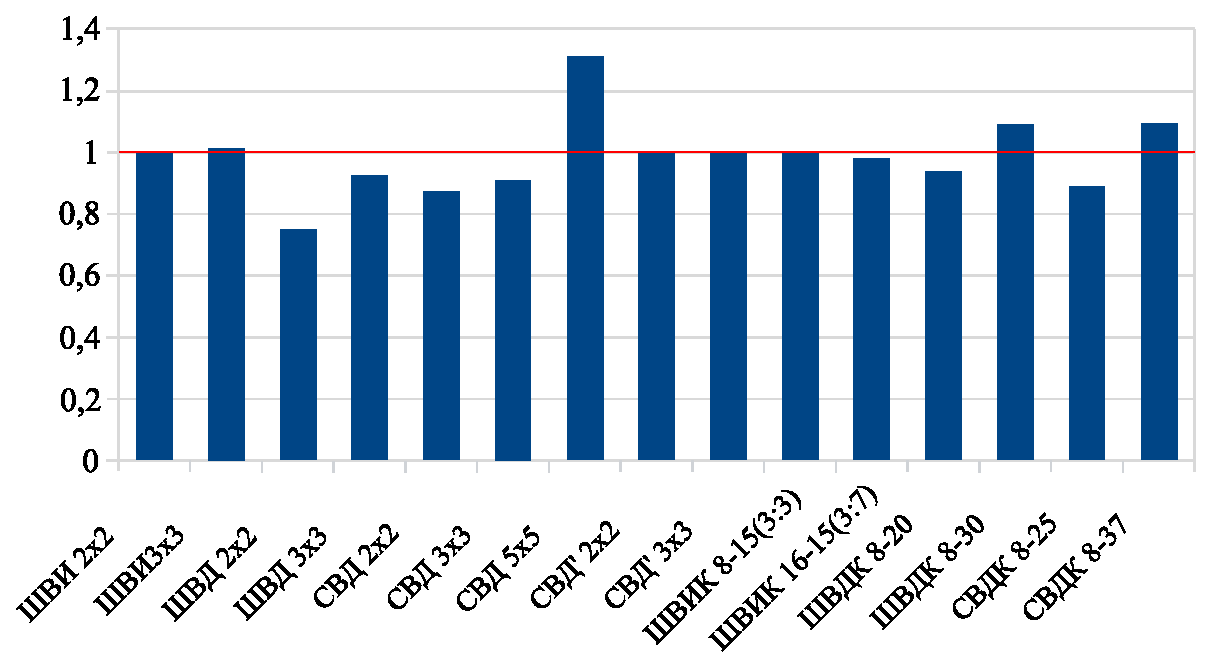
\includegraphics[width=0.95\linewidth]{ratio.eps}}
\caption{Отношение длительности вычислений с фиксацией первой координаты к исходной длительности вычислений}
\label{ris:time_ratio}
\end{figure}


Результаты данного раздела были представлены в~\cite{tyu:daor,tyu:motor,tyu:msim22}.
